\documentclass[a4paper,
fontsize=11pt,
%headings=small,
oneside,
numbers=noperiodatend,
parskip=half-,
bibliography=totoc,
final
]{scrartcl}

\usepackage{synttree}
\usepackage{graphicx}
\setkeys{Gin}{width=.4\textwidth} %default pics size

\graphicspath{{./plots/}}
\usepackage[ngerman]{babel}
\usepackage[T1]{fontenc}
%\usepackage{amsmath}
\usepackage[utf8x]{inputenc}
\usepackage [hyphens]{url}
\usepackage{booktabs} 
\usepackage[left=2.4cm,right=2.4cm,top=2.3cm,bottom=2cm,includeheadfoot]{geometry}
\usepackage{eurosym}
\usepackage{multirow}
\usepackage[ngerman]{varioref}
\setcapindent{1em}
\renewcommand{\labelitemi}{--}
\usepackage{paralist}
\usepackage{pdfpages}
\usepackage{lscape}
\usepackage{float}
\usepackage{acronym}
\usepackage{eurosym}
\usepackage[babel]{csquotes}
\usepackage{longtable,lscape}
\usepackage{mathpazo}
\usepackage[normalem]{ulem} %emphasize weiterhin kursiv
\usepackage[flushmargin,ragged]{footmisc} % left align footnote
\usepackage{ccicons} 
\setcapindent{0pt} % no indentation in captions

%%%% fancy LIBREAS URL color 
\usepackage{xcolor}
\definecolor{libreas}{RGB}{112,0,0}

\usepackage{listings}

\urlstyle{same}  % don't use monospace font for urls

\usepackage[fleqn]{amsmath}

%adjust fontsize for part

\usepackage{sectsty}
\partfont{\large}

%Das BibTeX-Zeichen mit \BibTeX setzen:
\def\symbol#1{\char #1\relax}
\def\bsl{{\tt\symbol{'134}}}
\def\BibTeX{{\rm B\kern-.05em{\sc i\kern-.025em b}\kern-.08em
    T\kern-.1667em\lower.7ex\hbox{E}\kern-.125emX}}

\usepackage{fancyhdr}
\fancyhf{}
\pagestyle{fancyplain}
\fancyhead[R]{\thepage}

% make sure bookmarks are created eventough sections are not numbered!
% uncommend if sections are numbered (bookmarks created by default)
\makeatletter
\renewcommand\@seccntformat[1]{}
\makeatother


\usepackage{hyperxmp}
\usepackage[colorlinks, linkcolor=black,citecolor=black, urlcolor=libreas,
breaklinks= true,bookmarks=true,bookmarksopen=true]{hyperref}
%URLs hart brechen
\makeatletter 
\g@addto@macro\UrlBreaks{ 
  \do\a\do\b\do\c\do\d\do\e\do\f\do\g\do\h\do\i\do\j 
  \do\k\do\l\do\m\do\n\do\o\do\p\do\q\do\r\do\s\do\t 
  \do\u\do\v\do\w\do\x\do\y\do\z\do\&\do\1\do\2\do\3 
  \do\4\do\5\do\6\do\7\do\8\do\9\do\0} 
% \def\do@url@hyp{\do\-} 
\makeatother 

%meta
%meta

\fancyhead[L]{K. Umlauf, S. Pohl\\ %author
LIBREAS. Library Ideas, 34 (2018). % journal, issue, volume.
\href{http://nbn-resolving.de/}
{}} % urn 
% recommended use
%\href{http://nbn-resolving.de/}{\color{black}{urn:nbn:de...}}
\fancyhead[R]{\thepage} %page number
\fancyfoot[L] {\ccLogo \ccAttribution\ \href{https://creativecommons.org/licenses/by/3.0/}{\color{black}Creative Commons BY 3.0}}  %licence
\fancyfoot[R] {ISSN: 1860-7950}

\title{\LARGE{Eine kurze Geschichte von Buch und Buchhandel
}}% title
\author{Konrad Umlauf \& Sigrid Pohl †} % author

\setcounter{page}{1}

\hypersetup{%
      pdftitle={Eine kurze Geschichte von Buch und Buchhandel
},
      pdfauthor={Konrad Umlauf \& Sigrid Pohl †},
      pdfcopyright={CC BY 3.0 Unported},
      pdfsubject={LIBREAS. Library Ideas, 34 (2018).},
      pdfkeywords={Buchmarkt, Erwerbung in Öffentlichen Bibliotheken},
      pdflicenseurl={https://creativecommons.org/licenses/by/3.0/},
      pdfcontacturl={http://libreas.eu},
      baseurl={http://libreas.eu},
      pdflang={de},
      pdfmetalang={de}
     }



\date{}
\begin{document}

\maketitle
\thispagestyle{fancyplain} 

%abstracts

%body
\hypertarget{die-anfuxe4nge}{%
\section{Die Anfänge}\label{die-anfuxe4nge}}

Das Buch entstand, als ein Bedarf aufgekommen war, Informationen
festzuhalten, die man sich ohne schriftliche Fixierung nicht gut merken
konnte. Das waren keineswegs Mythen und Epen. Die waren schon längst
mündlich überliefert; man konnte sie dank Reim und Rhythmus ordentlich
memorieren. Aber als in Mesopotamien, im Zweistromland Ende des 4.
Jahrtausends vor Christus eine so gute Bewässerung der Felder entwickelt
war, dass man ausgedehnte Vorräte anlegen und einen lebhaften Handel mit
Getreide und Olivenöl etablieren konnte, wollte man über Vorräte und
Handel den Überblick behalten -- das ging nur schriftlich. Die ersten
Bücher waren Geschäftsbücher und enthielten Lagerlisten, eine vielleicht
ernüchternde Erkenntnis. Man drückte mit einem Rohrgriffel keilförmige
Zeichen in weichen Ton. So entstand die Keilschrift auf Tontafeln. Damit
der Zusammenhang im Sinn eines Buches erkennbar blieb, nummerierte der
Schreiber die Tontafeln.

\begin{center}

\includegraphics{img/image1.jpg}
\end{center}

\hypertarget{buch-und-buchhandel-in-antike-und-mittelalter}{%
\section{Buch und Buchhandel in Antike und
Mittelalter}\label{buch-und-buchhandel-in-antike-und-mittelalter}}

Die Buchform der klassischen Antike war die Rolle aus Papyrus, manchmal
auch aus Pergament. Bereits in der Antike kam der Buchhandel auf:
Händler ließen beliebte Lesestoffe -- die berühmten Philosophen ebenso
wie wilde Abenteuergeschichten, Reiseberichte und schlüpfrige
Erzählungen -- durch Sklaven auf Vorrat abschreiben und boten sie auf
Marktständen neben gackernden Hühnern und Lederschläuchen voller Wein
an. Im 2. Jahrhundert nach Christus kam der Kodex auf -- das Buch in der
Form, wie wir es heute noch kennen: Blätter zwischen Buchdeckeln, die
links zusammengehalten werden. Üblicherweise bestanden die Blätter aus
Pergament. Der Kodex ist beim Lesen und Nachschlagen praktischer als die
Rolle. Er setzte sich bis zum 5. Jahrhundert wohl auch deshalb durch,
weil die Christen ihn bevorzugten. Ihnen galt die Schriftrolle als
heidnisches Relikt und außerdem hatte ihr Apostel Paulus nicht auf
Rollen geschrieben, sondern auf Wachstäfelchen, die bereits wie die
Blätter eines Kodex zusammengebunden waren. Bis zur Erfindung des
Buchdrucks um 1450 durch Johannes Gutenberg gab es nur handgeschriebene
Bücher. Ein tüchtiger Schreiber, meistens ein Mönch, brauchte ein Jahr,
um ein mäßig langes Buch von kaum mehr als 100 Seiten abzuschreiben. Das
Schriftbild war dann auch bezaubernd schön, sehr gleichmäßig -- fast wie
gedruckt -- und mit schmückenden Initialen versehen.

\hypertarget{gutenbergs-revolution}{%
\section{Gutenbergs Revolution}\label{gutenbergs-revolution}}

Dem Erfinder Gutenberg ging es nicht um das, was die Wirkung seiner
Erfindung war: die Rationalisierung der Buchherstellung, damit eine
enorme Preisreduktion und im Ergebnis die Verbreitung des Buches in
allen Schichten der Gesellschaft. Vielmehr wollte Gutenberg das
Schriftbild perfektionieren -- es sollte nicht sehr, sondern vollkommen
gleichmäßig sein. Der Witz an seiner Erfindung war nicht das Drucken --
Vervielfältigung durch Drucken von Holztafeln gab es schon vorher --,
sondern das Drucken mit beweglichen Lettern. Die Druckform wurde aus
Buchstabenkörpern, die aus einer Bleilegierung bestanden und meistens
ein, manchmal zwei Buchstaben trugen, zusammengesetzt. Nach dem Druck
legte man die Lettern in den Setzkasten zurück und konnte sie für eine
andere Buchseite wieder zusammensetzen. Mit Gutenbergs Innovation
vergleichbare Erfindungen im Korea des 12. Jahrhunderts und schon im
Jahr 1045 in China erzielten keinen Durchbruch, weil die damaligen
asiatischen Gesellschaften kein Interesse an Textvervielfältigung im
großen Stil hatten. Das war zu Gutenbergs Zeiten ganz anders: Humanismus
und Renaissance hatten ein brennendes Interesse daran, die antiken
Texte, die oft nur in ganz wenigen Handschriften überliefert waren und
fast unerreichbar in Klosterbibliotheken lagen, neu herauszugeben. Der
Papst ließ massenweise Ablassbriefe drucken und verkaufen, um den Neubau
des Petersdoms in Rom zu finanzieren. Dagegen zog Luther zu Felde und
die Reformation entzündete ein nie vorher dagewesenes Verlangen nach
Textvervielfältigung: Man wollte jetzt nicht nur den Priester hören,
sondern selbst in der Bibel lesen, und vor allem war man begierig auf
die Bibelauslegung der Reformatoren.

Gutenberg war Verleger, Setzer, Drucker und Bucheinzelhändler in einer
Person. Ab 1480 löste sich der Vertrieb von der Herstellung: Reisende
\emph{Buchführer} übernahmen die Verbreitung an die Endkunden. Sie
hatten naturgemäß nur ein schmales Sortiment dabei. Deshalb reiste das
gelehrte -- und vermögende -- Publikum einmal im Jahr zu Buchmessen in
Frankfurt am Main, in Leipzig, Venedig, Florenz, Oxford, Cambridge und
Paris oder man schickte seine Beauftragten dorthin. Erst im späten 18.
Jahrhundert waren das Interesse an Büchern -- jetzt konnte fast ein
Viertel der Bevölkerung lesen -- und die Kaufkraft so angestiegen, dass
sich ein stationärer Bucheinzelhandel etablieren konnte.

\hypertarget{viele-kleine-innovationen-im-19.-und-20.-jahrhundert}{%
\subsection{Viele kleine Innovationen im 19. und 20.
Jahrhundert}\label{viele-kleine-innovationen-im-19.-und-20.-jahrhundert}}

Statt einer einzigen umwälzenden Neuerung wie Gutenbergs Erfindung waren
es im 19. und 20. Jahrhundert viele kleine Schritte, die zusammen dazu
führten, dass die Buchbranche sich neu aufstellte:

\begin{itemize}
\item
  Die Schnellpresse, 1811 von Friedrich Koenig erfunden, beschleunigt
  den Buchdruck um den Faktor drei bis zwölf, indem eine Walze die Bögen
  einzieht, statt dass sie einzeln händisch in die Druckerpresse
  eingelegt werden. Die Schnellpresse und weitere Optimierungen der
  Buchherstellung führen zu Preisreduktionen der Bücher, so dass der
  Buchmarkt spätestens seit der Mitte des 20. Jahrhunderts als echter
  Massenmarkt gelten kann.
\item
  Aber erst 1884 wird das händische Zusammensetzen der Druckform aus
  einzelnen Lettern durch Satzmaschinen (Linotype) abgelöst. Heute hat
  der computergestützte Satz alle älteren Satzverfahren verdrängt.
\item
  Wer zur Zeit Goethes ein Buch kaufte, erstand einen Buchblock ohne
  Einbanddecke, ging damit zum Buchbinder und ließ einen Bucheinband
  anfertigen. Das erlaubt zwar, dem eigenen Geschmack, passend zur
  Wohnungseinrichtung, Geltung zu verschaffen, taugt aber nicht für den
  Massenmarkt. Erst seit der Mitte des 19. Jahrhunderts setzt sich der
  Verlagseinband durch.
\item
  Der Durchbruch des Taschenbuchs in der zweiten Hälfte des 20.
  Jahrhunderts (zuerst 1935 in Großbritannien mit den \emph{Penguin
  Books}) bringt einen weiteren großen Schritt in den Massenmarkt.
\item
  Gegen das Buch als Massenware entstehen seit 1890 immer wieder
  innovative Ansätze des Buchdesigns und Buchkunstbewegungen. Verleger
  und Buchgestalter wie William Morris, Eugen Diederichs, Emil Rudolf
  Weiß, Franz Greno, Roswitha Quadflieg oder Judith Schalansky geben dem
  Buch ein hochwertiges Design in Typografie, Layout, Illustration und
  Material.
\item
  1825 gründen Verleger und Buchhändler mit dem \emph{Börsenverein der
  Deutschen Buchhändler} (heute: \emph{Börsenverein des Deutschen
  Buchhandels}) den ersten überregionalen Unternehmensverband. Er kämpft
  gegen Zensur, rationalisiert das Handelsgeschäft mit der Schaffung der
  \emph{Verkaufsordnung} und der \emph{Verkehrsordnung}, den ersten
  Allgemeinen Geschäftsbedingungen des Buchhandels, und gründet 1912 in
  Leipzig und nach der deutschen Teilung 1947 in Frankfurt am Main die
  Vorgänger der heutigen \emph{Deutschen Nationalbibliothek} mit dem
  Auftrag, die gesamte deutsche und deutschsprachige Buchproduktion zu
  sammeln und für die Nachwelt aufzubewahren.
\item
  Nach einer Phase des ruinösen Preiswettbewerbs, in dem Verleger gegen
  Einzelhändler stehen, Buchhändler in urbanen Zentren gegen die
  Provinzialbuchhändler in kleinen Städten, wirtschaftsliberal denkende
  Großverleger gegen rückwärtsgewandt-zünftig eingestellte
  Sortimentsbuchhändler, rauft sich die Branche zur Buchpreisbindung
  durch: Die Mitglieder des Börsenvereins verpflichten sich 1888, den
  vom Verlag festgesetzten Endverkaufspreis einzuhalten. Wer sich nicht
  daran hält, wird nicht beliefert. Maßgeblichen Anteil an der nach ihm
  benannten Reform hat der Stuttgarter Verleger Adolf Kröner; sein
  Verlag existiert bis heute. 2002 wird die Buchpreisbindung mittels
  brancheninterner Vereinbarungen durch das Buchpreisbindungsgesetz
  abgelöst.
\item
  1843 gab es in Deutschland 883 Sortimentsbuchhandlungen, 1880 waren es
  3.375, 1929 allein in Berlin 524 -- ein Fünftel aller deutschen
  Sortimentsbuchhandlungen. Krieg und Inflation hatten ihre Spuren
  hinterlassen. Heute ist die Buchhandelsdichte in Deutschland im
  internationalen Vergleich außerordentlich hoch -- auch dank der
  Buchpreisbindung, die einen vermutlich ruinösen Preiswettbewerb
  verhindert.
\item
  Neben den stationären Buchhandlungen gehörten zur Buchbranche vom 18.
  bis in die Mitte des 20. Jahrhunderts Unternehmen, die Bücher nicht
  verkauften, sondern vermieteten: Leihbüchereien. Sie unterschieden
  sich von Bibliotheken der öffentlichen Hand (Öffentliche Bibliotheken,
  Universitäts-, Staatsbibliotheken und so weiter) durch ihr
  unternehmerisches Geschäftsmodell. Die Mietzahlungen der Kunden
  mussten mindestens die Kosten decken. Sie erreichten insgesamt mehr
  Kunden aus allen Schichten der Gesellschaft als die stationären
  Buchhandlungen; das reiche Bürgertum und der Adel schickten die
  Dienstboten, die für ihre Herrschaften auch Bücher holten. Steigende
  Einkommen der Kunden und die Verbilligung der Buchpreise entzogen
  ihnen die Geschäftsgrundlage. Im digitalen Zeitalter kehrt dieses
  Geschäftsmodell in Form von Flatrates für die E-Book-Nutzung von
  Anbietern wie Amazon (Kindle Unlimited) oder Skoobe zurück.
\item
  Als im 19. Jahrhundert das Lesen von Büchern unter Jugendlichen selbst
  auf dem Land üblich wurde, warnten Pädagogen vor der Lesewut und
  wollten den Nachwuchs lieber zum Spielen auf die grüne Wiese schicken
  -- ohne Erfolg. Heute sehen Pädagogen die Lesekompetenz in Gefahr und
  fordern Aktionen zur Leseförderung -- wenn es gut geht gemeinsam mit
  dem Buchhandel.
\item
  Bedrückend waren für Autoren wie Verleger jahrhundertelang die
  Raubdrucke -- ein vor Einführung des Urheberrechtsschutzes legaler
  \enquote{geistiger Diebstahl}. 1837 führen Preußen und der Deutsche
  Bund erstmals einen Urheberrechtsschutz ein -- in England ist er seit
  1710 etabliert. Ein erstes gesamtdeutsches Gesetz, der Vorläufer des
  heutigen Urheberrechtsgesetzes, tritt 1871 in Kraft. Der Börsenverein
  erringt mit ihm einen aus seiner Sicht bedeutenden Erfolg.
\item
  Innovative Vertriebswege (Buchhandelsabteilungen in Warenhäusern seit
  dem späten 19. Jahrhundert; Taschenbuchdrehsäulen in Tankstellen,
  Lebensmittelfilialen und Apotheken und anderes mehr) machen Bücher
  überall da greifbar, wo Kunden erscheinen, die zunächst gar nicht an
  Buchkauf denken.
\end{itemize}

\hypertarget{vier-haupttendenzen-seit-gutenberg}{%
\section{Vier Haupttendenzen seit
Gutenberg}\label{vier-haupttendenzen-seit-gutenberg}}

Es wird deutlich, dass Teile der Buchbranche jeweils etliche dieser
Schritte negativ werten; es ist eine Frage der Perspektive und der
Betroffenheit. Zum Beispiel sieht der Sortimentsbuchhandel im
Vertriebskanal Apotheken einen Kaufkraftabfluss, während die Verlage
hierin die Chance der Umsatzsteigerung sehen. Oder die Digitalisierung
der Buchherstellung hat den traditionsreichen Beruf des Setzers
vernichtet. Er ist seit 1998 durch den Beruf Mediengestalter Digital und
Print abgelöst, hat jedoch mit Texterfassung Buchstabe für Buchstabe
kaum noch etwas zu tun. In Krisenzeiten tritt die Buchbranche nicht
verstärkt solidarisch auf, sondern Partikularinteressen werden lauter
artikuliert und durchgesetzt. Seit Gutenberg war die Geschichte des
Buches und des Buchhandels von vier Haupttendenzen geprägt:

\begin{itemize}
\item
  Bücher wurden immer billiger. Zu Gutenbergs Zeiten kostete eine seiner
  wertvollen Inkunabeln so viel wie ein Stadthaus. Ein Facharbeiter
  musste um 1900 eine Stunde arbeiten, um sich ein Reclamheft leisten zu
  können -- heute hat er in sieben Minuten die Kaufkraft für ein
  Reclamheft erworben. Und vor allem: Um 1900 war, wenn Miete und
  Kohlen, Lebensmittel und Tanzvergnügen am Wochenende bezahlt waren,
  kaum noch etwas übrig, von dem man sich hätte Bücher kaufen können.
  Heute sind zwei Drittel der Frauen und die Hälfte der Männer
  Buchhandelskundinnen und -kunden. 47 Prozent der Personen in
  Haushalten bis 1.000 Euro Monatsnettoeinkommen kaufen regelmäßig
  Bücher. Die Ursache für diese Verbilligung sind technische
  Innovationen in der Buchherstellung.
\item
  Bücher haben die Gesellschaft immer mehr durchdrungen. Sie fanden
  immer mehr Kunden und Leser. Hier spielt auch eine Rolle, dass seit
  Beginn des 20. Jahrhunderts der Analphabetismus eine marginale Rolle
  spielt. In der Gegenwart sind Bücher historisch erstmals
  allgegenwärtig: Jedes Schulkind kommt mit Büchern in Kontakt, fast
  jeder Haushalt besitzt Bücher, das Netz der stationären Buchhandlungen
  ist dicht und darüber hinaus kann man an vielen weiteren
  Verkaufsstellen von Lebensmittelmärkten bis zu Tankstellen Bücher
  kaufen. Drei von vier Erwachsenen greifen mehr oder minder regelmäßig
  zum Buch.
\item
  Immer öfter überschreiten Bücher und Buchinhalte politische und
  Sprachgrenzen. Schon im 17. Jahrhundert waren die Buchmessen erst in
  Frankfurt am Main, dann in Leipzig internationale Umschlagplätze für
  Bücher. Vor 25 Jahren gab es wenige Sortimentsbuchhandlungen, meistens
  nur in Universitätsstädten, die ausländische Literatur besorgen
  konnten. Heute gehört dies zum Alltagsgeschäft mehr oder minder jeder
  Sortimentsbuchhandlung. In Deutschland erscheinen jedes Jahr rund
  12.000 Übersetzungen aus anderen Sprachen.
\item
  Bücher und Buchhandel haben sich immer wieder gewandelt, haben
  Umbrüche erlebt und hervorgebracht. Ihre Geschichte ist von Neuerungen
  und von Verschiebungen innerhalb der Branche geprägt, eine spannende
  Geschichte. Wer sie erfolgreich fortführen möchte, braucht
  Innovationskraft im Geist, Ruhe in der Seele und Tatkraft im Handeln.
  Bei all diesem Wandel ging und geht es darum, den Kern des Geschäfts
  -- die gesellschaftliche Kommunikation über Schriftmedien auf Basis
  unternehmerischen Handelns -- jeweils zeitgemäß zu organisieren und
  ihm Mehrwerte zu geben, die über die Logistik hinausgehen, zeitgemäß
  sowohl in technischer und kultureller Hinsicht (Papier, Ausstattung,
  digitale Ausgaben; das Buch als Statussymbol oder als
  Alltagsgegenstand) wie auch hinsichtlich der Geschäftsmodelle
  (inhabergeführte Sortimentsbuchhandlungen, Filialisten,
  internetbasierter Versandhandel; Buchhandlungen als Schmökerstuben
  oder als Bühne des Lifestyles und so weiter).
\end{itemize}

\begin{center}
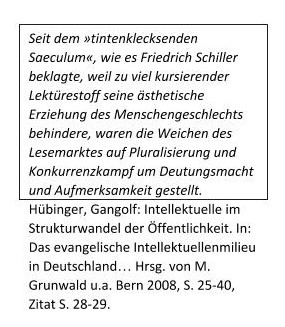
\includegraphics{img/image2.jpg}
\end{center}

\hypertarget{perspektiven-des-buchs-und-des-buchhandels-im-21.-jahrhundert}{%
\section{Perspektiven des Buchs und des Buchhandels im 21.
Jahrhundert}\label{perspektiven-des-buchs-und-des-buchhandels-im-21.-jahrhundert}}

Am Ende des 20. und im frühen 21. Jahrhundert stehen Trends im
Vordergrund, die sich mit dem Stichwort Digitalisierung zusammenfassen
lassen:

\begin{itemize}
\item
  Die Buchherstellung beruht heute fast überall auf
  Informationstechnologie. Die Autoren liefern kein Papier an den
  Verlag, sondern Dateien. In immer mehr Verlagen werden die Werke --
  Texte, Bilder, Layout-Anweisungen -- in einer XML-Datenbank
  vorgehalten, aus der heraus Ausgabeformate für den Druck und für die
  Online-Publikation automatisch generiert werden. Wenn gedruckt wird,
  dann immer häufiger im Digitaldruck, besonders bei kleinen Auflagen.
\item
  Das Blättern in gedruckten Buchhandelskatalogen gehört der
  Vergangenheit an. Kunden und Buchhändler recherchieren in Datenbanken
  und senden die Bestellung über das Internet an den Lieferanten. Wenn
  der Kunde daheim selbst recherchiert, dann noch zu selten auf der
  Website seiner örtlichen Sortimentsbuchhandlung, obwohl sie dasselbe
  Lieferpotential wie Amazon und andere große Versandbuchhandlungen
  haben kann, in vielen Fällen ein besseres Lieferpotential, wenn
  nämlich die Buchhändler ausländische und antiquarische Verzeichnisse
  mit einbeziehen. Und sie kann schneller liefern, wenn sie die Logistik
  der Barsortimente nutzt. Aber viele Kunden wissen das nicht. Hier
  müssen die einzelnen Buchhandlungen und vor allem der Börsenverein die
  Öffentlichkeit besser informieren.
\item
  Sobald die Ware in der Buchhandlung eingetroffen ist, wird der Vorgang
  im Warenwirtschaftssystem erfasst. Auch Lieferschein und Rechnung
  kommen über das Internet. Jeder Verkaufsvorgang wird im Computer
  abgebildet. Die Buchhandlung hat auf diese Weise so tiefe und
  differenzierte Daten über Lagerhaltung und Verkauf, wie es ohne
  Informationstechnik nicht denkbar wäre. Jetzt muss sie die Daten auch
  nutzen, um sowohl Ballast wie auch Lücken im Lager zu vermeiden. Wenn
  die Buchhandlung ihrerseits Rechnungen für die Kunden ausstellt, holt
  sie die benötigten Daten -- Kundenstammdaten, Titelangaben, Anzahl und
  Preis -- wiederum aus dem Warenwirtschaftssystem. Das
  Warenwirtschaftssystem übergibt die Daten der Buchhaltung, die
  ihrerseits mittels Computer erfolgt.
\item
  Aber eigentlich muss der Kunde gar nicht mehr in die Buchhandlung
  kommen, um das bestellte Buch abzuholen. Er kann ein E-Book beziehen
  und muss dazu nicht mal die Wohnung verlassen. Bisher hat der
  Sortimentsbuchhandel am Vertrieb digitaler Bücher einen marginalen
  Anteil. Aber er hat Stärken, die kein Anbieter von E-Books im Internet
  wettmachen kann. Der Sortimentsbuchhandel kann ein Einkaufserlebnis
  vermitteln, das vom inspirierenden Ambiente über das Treffen mit
  Freunden und dem Gespräch über Leseerlebnisse mit der Buchhändlerin
  bis zum Latte macchiato reicht. Bei der künftigen Profilierung des
  Sortimentsbuchhandels müssen diese Funktionen, die über die Logistik
  hinausgehen, im Fokus stehen, Funktionen, die den Sortimentsbuchhandel
  einzigartig machen. Auch die Digital Natives -- und die womöglich noch
  stärker als mancher Rentner, der nie ein E-Book kaufen wird -- suchen
  Erlebnisse in der realen Welt, unmittelbare Kontakte zu anderen
  Menschen und fläzen sich gerne in solchen Sesseln, die sie zuhause
  nicht haben. Vielleicht verkauft die Sortimentsbuchhandlung der
  Zukunft mehr Aufenthaltsqualität als Bücher\ldots{}
\end{itemize}

%autor

\end{document}
